% !TEX root = ../coursera_sc_01.tex

\begin{frame} % название фрагмента

\videotitle{Wiener process}

\end{frame}


\begin{frame}{Stochastic calculus course}
  The goal: price an option in the framework of Black and Scholes model. 

  \begin{itemize}[<+->]
    \item Very short: \alert{4 weeks} only.
    \item Mathematics is \alert{hard}.
    \item \alert{Informal} definitions and theorems. 
    \item \alert{Problem solving} and computer \alert{simulations}. 
  \end{itemize}

\end{frame}


\begin{frame}{Wiener process}

  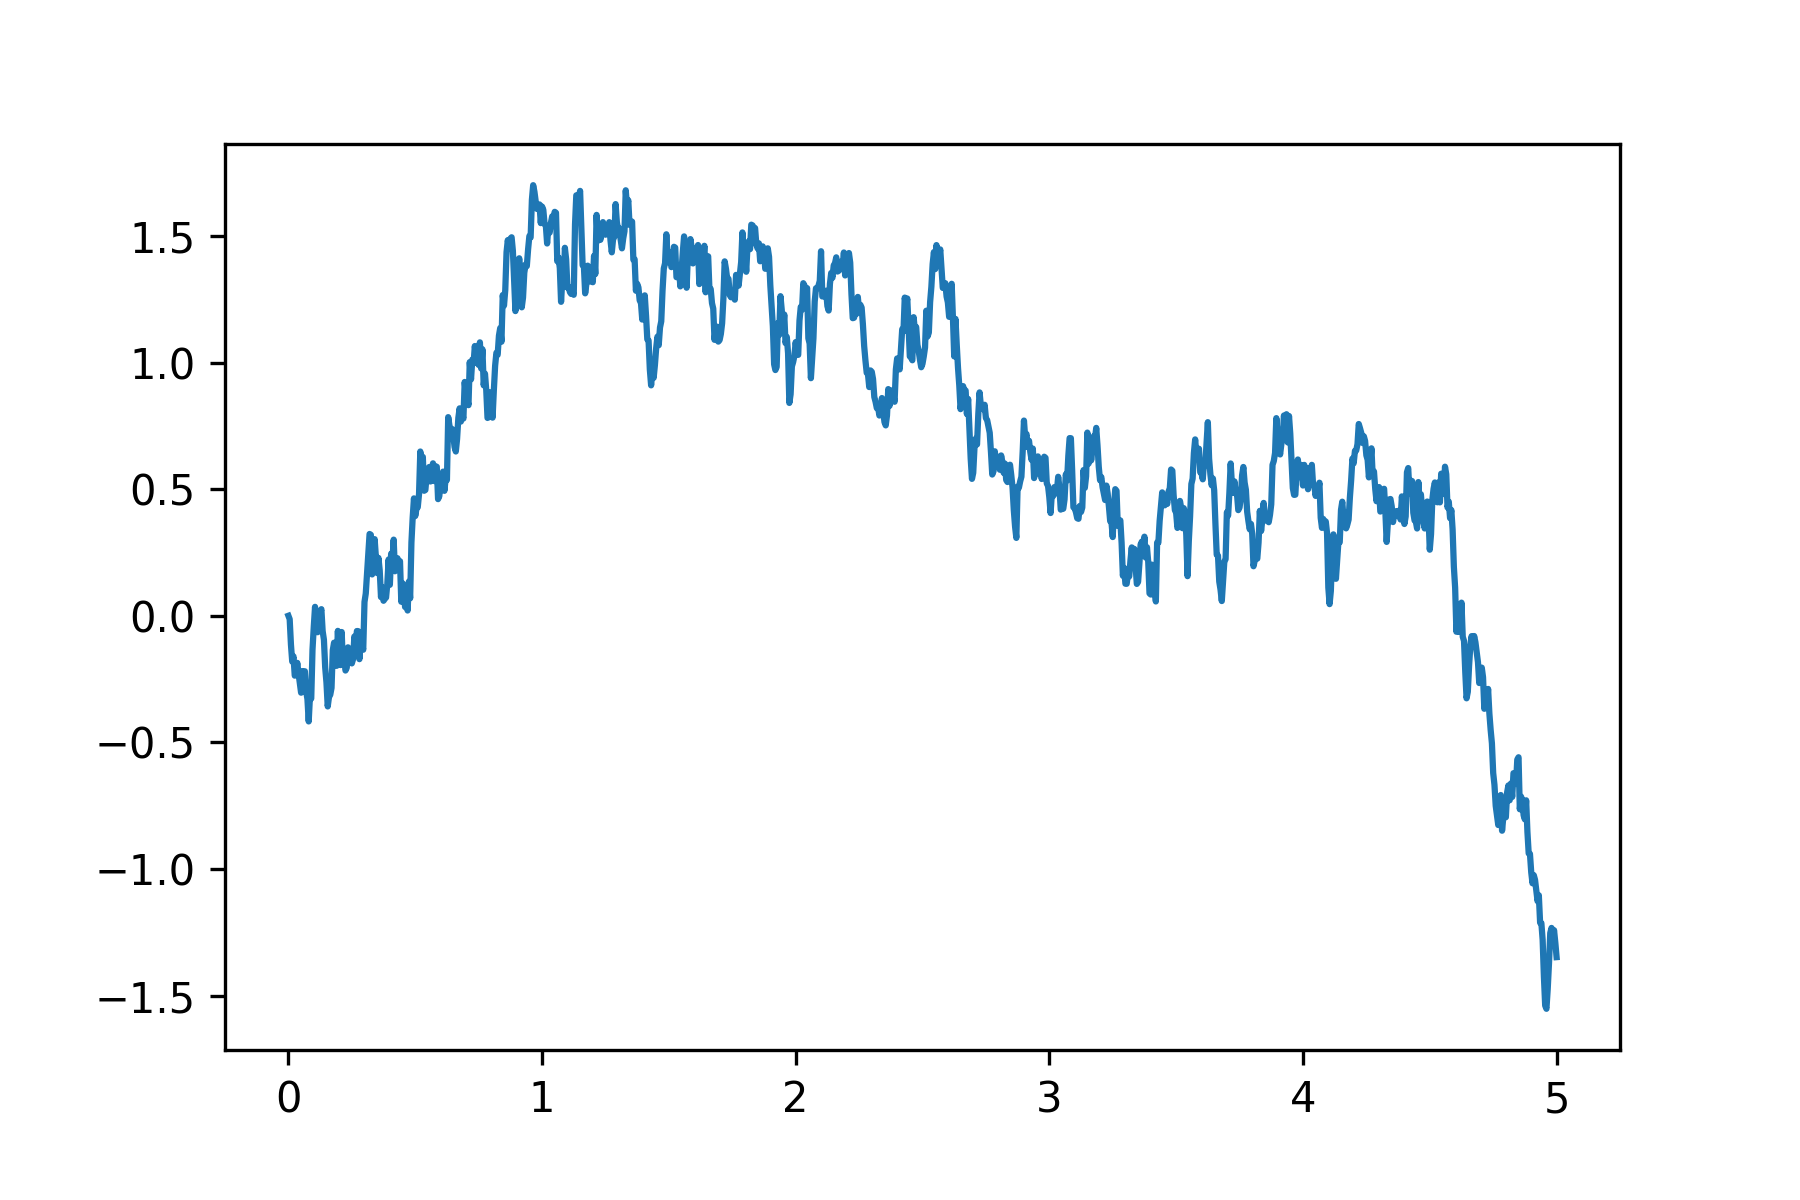
\includegraphics[width=\textwidth]{pictures/wiener_process.png}


\end{frame}


\begin{frame}{Stochastic process}

  \begin{block}{Definition \formalduck}
    \alert{Stochastic} or \alert{random process} is a collection of random variables indexed by time variable $t$. 
    \pause

    \alert{Continuous time}: $(X_t, t\geq 0)$.
    \pause 
    
    \alert{Discrete time}: $(X_t, t\in \{0, 1, 2, 3, \ldots \})$. 
\end{block}

\pause 
Notation remark:
\begin{itemize}[<+->]
  \item $(X_t, t\geq 0)$ or $(X_t)$ — collection of random variables;
  \item $X_t$ — one particular random variable. 
\end{itemize}


\end{frame}

\begin{frame}
  \frametitle{Wiener process}

  \begin{block}{Definition\formalduck}
    Stochastic process $(W_t, t\geq 0)$ is called \alert{Wiener process} or \alert{Brownian motion} if 
    \pause
    \begin{enumerate}[<+->]
      \item $W_0 = 0$.
      \item Increments $W_t - W_s$ are normally distributed $\cN(0; t-s)$. 
      \item Increment $W_t - W_s$ is independent of the past values $(W_u, u\leq s)$.
      \item $\P(\text{trajectory of } (W_t) \text{ is continuous} ) = 1$.
  \end{enumerate}
  
  \end{block}

  \pause 
  Tradition: when we consider two arbitrary moments of time, $s$ and $t$, we usually assume $s \leq t$. 
\end{frame}

\begin{frame}
  \frametitle{Divide and conquer}

  The main trick to study properties:
  \[
  \text{\alert{Future value}} = \text{\alert{Known value}} + \text{\alert{Unpredictable change}}  
  \]
  \pause 
  Seems trivial\harlequinduck
  \[
  W_t = W_s + (W_t - W_s)  
  \]

\end{frame}


\begin{frame}
\frametitle{Conditional probability exercise}
Exercise\knightduck. Calculate $\P(W_{10} > 2 \mid W_6 = 3)$.
\begin{align*}
  \onslide<2->{&\P(W_{10} > 2 \mid W_6 = 3) = \P(W_{10} - W_6 + W_6 >2 \mid W_6 = 3) = } \\
  \onslide<3->{&= \P(W_{10} - W_6 + 3 >2 \mid W_6 = 3) = \P(W_{10} - W_6 > -1)}.
\end{align*}
\[
\onslide<4->{W_{10} - W_6 \sim \cN(0;4), \pause \text{ hence } \frac{W_{10} - W_6 - 0 }{\sqrt{4}} \sim \cN(0;1)}. 
\]

\onslide<5->{We will use standard normal distribution function $F(u) = \P(Z \leq u)$, where $Z\sim \cN(0;1)$.}
\begin{align*}
  \onslide<6->{\P(W_{10} - W_6 > -1) = \P\left(\frac{W_{10} - W_6}{2} > -\frac{1}{2}\right)  = }\\
  \onslide<7>{= \P(Z > -0.5) = \P(Z < 0.5) = F(0.5) \pause \approx 0.69.}
\end{align*}


\end{frame}


\begin{frame}
  \frametitle{More gentlemen's agreements}

  On slides we will follow these agreements:
  \begin{itemize}[<+->]
    \item $s$ and $t$ denote two arbitrary time moments with $0 \leq s \leq t$.
    \item $(W_t)$ denotes a Wiener process.
    \item $Z$ denotes a standard normal random variable, $Z \sim \cN(0;1)$.
    \item $F(u)$ denotes the standard normal distribution function, $F(u) = \P(Z \leq u)$.
  \end{itemize}
  

\end{frame}



\begin{frame}
  \frametitle{Independence of increments: example}
  \begin{block}{Property}
    Increment $W_t - W_s$ is independent of the past values $(W_u, u\leq s)$.  
  \end{block}

  \pause 
  $W_6 - W_4$ is independend of $W_4$, $W_{3}$, $W_{2.5}$, $W_1$, \ldots 

  \pause 
  $W_6 - W_4$ is independent of $W_4 - W_3$, $W_{2.5} - W_{1}$.

  \pause
  The increments $W_6 - W_4$, $W_4 - W_3$, $W_{2.5} - W_1$ are independent. 

\end{frame}


\begin{frame}
  \frametitle{Independence of increments: full glory}


  If the time intervals $[s_1, t_1]$, $[s_2, t_2]$, \ldots, $[s_k, t_k]$ are
  \alert{non overlapping},

  \begin{center}
    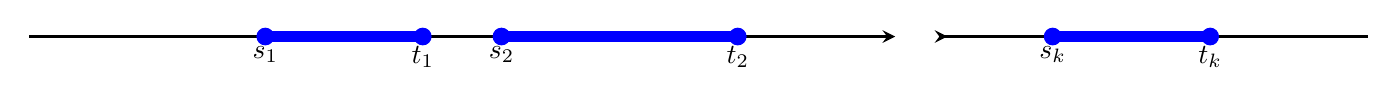
\begin{tikzpicture}
      \coordinate (a) at (-3,0);
      \coordinate (b) at (14,0);

      \coordinate [label=below:$s_1$] (s1) at (0,0);
      \coordinate [label=below:$t_1$] (t1) at (2,0);
      \coordinate [label=below:$s_2$] (s2) at (3,0);
      \coordinate [label=below:$t_2$] (t2) at (6,0);
      \coordinate [label=below:$s_k$] (sn) at (10,0);
      \coordinate [label=below:$t_k$] (tn) at (12,0);  



      \draw[line width=1pt, black, -stealth] (a)--(8,0);
      \draw[line width=1pt, black, stealth reversed-] (8.5,0)--(b);

      \filldraw [blue] (s1) circle[radius=3pt];
      \filldraw [blue] (t1) circle[radius=3pt];
      \filldraw [blue] (s2) circle[radius=3pt];
      \filldraw [blue] (t2) circle[radius=3pt];
      \filldraw [blue] (sn) circle[radius=3pt];
      \filldraw [blue] (tn) circle[radius=3pt];

      \draw[line width=4pt, blue] (s1)--(t1);
      \draw[line width=4pt, blue] (s2)--(t2);
      \draw[line width=4pt, blue] (sn)--(tn);     
    \end{tikzpicture}
  \end{center}
  

  \pause 
  then the increments $W(t_1) - W(s_1)$, $W(t_2) - W(s_2)$, \ldots, $W(t_k) - W(s_k)$ are independent. 

  \pause
  Remark: the right border of an interval \alert{may touch} the left border of the next one,
  but \alert{may not exceed} it, $t_j \leq s_{j+1}$. 

\end{frame}


\begin{frame}
  \frametitle{Expectation and variance}

  Exercise\knightduck. Find $\E(W_t)$, $\Var(W_t)$, $\Cov(W_s, W_t)$.
  \begin{flalign*}
    \onslide<2->{\E(W_t) &= \E(W_t - W_0) = 0&}    
  \end{flalign*}
  \begin{flalign*}
  \onslide<3->{\Var(W_t) &= \Var(W_t - W_0) = t - 0 = t&}
\end{flalign*}  
  \onslide<4->{For $t\geq s$:}
  \begin{flalign*}  
  \onslide<5->{\Cov(W_s, W_t) &= \Cov(W_s, W_s + (W_t - W_s)) = \Cov(W_s,W_s) = s&}
\end{flalign*}
\begin{flalign*}
    \onslide<6>{\Cov(W_7, W_3) &= 3.&}  
  \end{flalign*}

\end{frame}


\begin{frame}{Two friends}

  \begin{block}{Definition\formalduck}
    Stochastic process $(X_t, t\geq 0)$ that may be written as
    \[
    X_t = a W_t + b t,  
    \]
    is called \alert{brownian motion with drift and scaling}.
  \end{block}

  \pause
  \begin{block}{Definition\formalduck}
    Stochastic process $(S_t, t\geq 0)$ that may be written as
    \[
    S_t = S_0 \exp(a W_t + b t),
    \]
    is called \alert{geometric brownian motion}.
  \end{block}
  
\end{frame}


\begin{frame}{Two plots}

  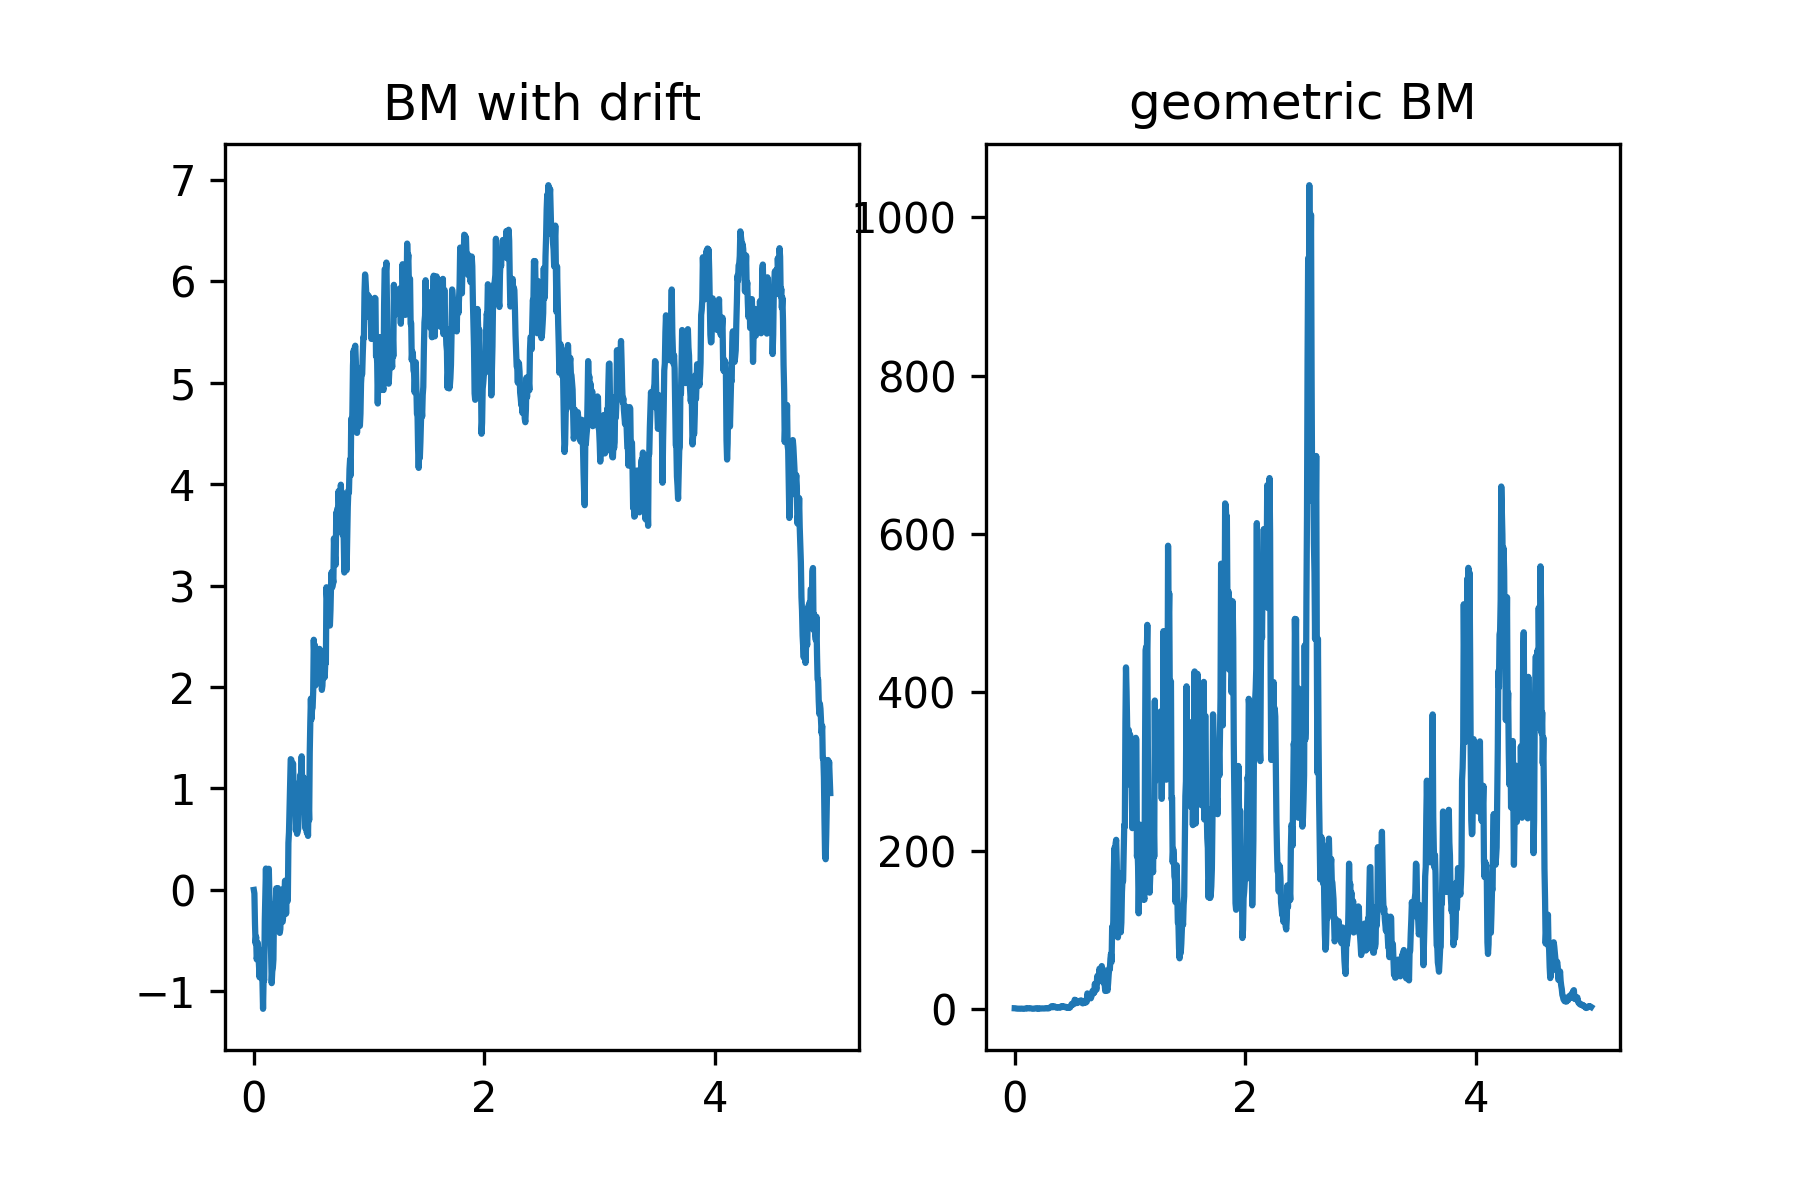
\includegraphics[width=\textwidth]{pictures/two_wiener_friends.png}

\end{frame}


\begin{frame}
  \frametitle{BM with drift and scaling}

  Exercise\knightduck. Find $\E(5W_t + 6t)$ and $\Var(5W_t + 6t)$.
  
  \begin{flalign*}    
  \onslide<2->{\E(5W_t + 6t) &= 0 + 6t = 6t&}
  \end{flalign*}
  \begin{flalign*}    
    \onslide<3->{\Var(5W_t + 6t) &= \Var(5W_t) = 25t&}
  \end{flalign*}

\end{frame}

\begin{frame}
  \frametitle{Frequently used expected values}

  \onslide<1->{Expected values of exponents:}
  \pause
  \begin{itemize}[<+->]
    \item $\E(\exp(aZ)) = \exp(a^2/2)$ for $Z \sim \cN(0;1)$.
    \item $\E(\exp(aW_t)) = \exp(a^2t/2)$ for Wiener process $W_t$.
  \end{itemize}
  
  \onslide<4->{
  \begin{block}{How these are obtained?\formalduck}
    \pause
    \begin{flalign*}
      \E(\exp(aZ)) &= \int_{-\infty}^{+\infty} \exp(az) f(z) \,dz = &\\
      & = \int_{-\infty}^{+\infty} \exp(az) \frac{1}{\sqrt{2\pi}}\exp(-z^2/2) \,dz&
    \end{flalign*}
  \end{block}
  }

\end{frame}


\begin{frame}
  \frametitle{Moment generating function}

\begin{block}{Definition\formalduck}
  The \alert{moment generating function} (MGF) of a random variable $X$ is defined as 
  \[
  M_X(a) = \E(\exp(a X)).
  \] 
\end{block}

\pause 

\begin{itemize}[<+->]
  \item $M_Z(a) = \exp(a^2/2)$ for a normal $Z \sim \cN(0;1)$.
  \item $M_{W_t}(a)= \exp(a^2t/2)$ for a Wiener process $W_t$.
\end{itemize}
  
\end{frame}

\begin{frame}
    \frametitle{Why may we need MGF?}
    \[
    \onslide<1->{M'(u) = \frac{d}{du}\E(\exp(uX)) =\E(X\exp(uX)) }
    \]
    \[
    \onslide<2->{M'(0) = \E(X)}  
    \]
    \onslide<3->{MGF is a funny\harlequinduck { } way to calculate expected value!}
    \begin{align*}
      \onslide<4->{M''(0) &= \E(X^2)& } \\
      \onslide<5->{M'''(0) &= \E(X^3)&  } \\
      \onslide<6->{&\vdots}      \\
      \onslide<7->{M^{(k)}(0) &= \E(X^k)&}      
    \end{align*}
  
  \end{frame}

\begin{frame}{Wiener process: summary}

\begin{itemize}[<+->]
    \item Stochastic process with \alert{normal} and \alert{independent increments}.
    \item Wiener process with \alert{drift} and \alert{geometric Wiener process}. 
    \item \alert{Moment generating function}. 
\end{itemize}
  
\end{frame}
